\documentclass[pdf, fyma2]{prosper}
\usepackage[czech]{babel}
\usepackage[utf8]{inputenc}

\usepackage{graphicx}

\DefaultTransition{Replace}

\begin{document}

  \title{ITY\,--\,Projekt č. 5}
  \subtitle{Stručná pravidla tenisu}
  \author{Martin Janyš}
  \email{xjanys00@stud.fit.cz}
  \date{2011}
  
  \maketitle

\begin{slide}{Úvod}
  \begin{itemize}
    \item{Hra tenis vznikla v Anglii}
    \item{Tenis patří k olympijským sportům}
    \item{Z tenisu se vyvinulo několik podobných sportů}
    \begin{itemize}
      \item{squash}
      \item{ricochet}
      \item{plážový tenis} 
    \end{itemize}
  \end{itemize}
\end{slide}

\overlays{2}{
\begin{slide}{Pravidla}
  \begin{itemize}
    \item{Základem tenisu je dostat míč (tenisák) přes síť do soupeřovy části hřiště}
    \item{Hraje se na maximálně jeden dopad a míč musíte dostat na druhou stranu jedním úderem}
    \item{Pokud ho soupeř nedokáže obdobným způsobem vrátit, je to váš vítězný míč}
    \item{Špatný míč}
    \fromSlide{2}{
    \begin{itemize}
      \item{míč spadne dvakrát na zem na vaší polovině} 
      \item{přesáhnete raketou přes síť na soupeřovu polovinu}
      \item{hrajete-li v hale a trefíte strop} 
      \item{přijímáte-li podání a trefíte ho před dopadem na zem} 
    \end{itemize}
    }
  \end{itemize}
\end{slide}}

\overlays{2} {
\begin{slide}{Počítání}
  \begin{itemize}
    \item{Získá-li hráč bod, je stav 15:0}
    \item{Získá-li druhý, je stav 30:0} 
    \item{Získá-li třetí, je stav 40:0}
    \item{Získá-li čtvrtý bod, vyhrává hru}
    \item{Pokud je stav 40:40, tzv. shoda}
    \fromSlide{2} {
    \begin{itemize}
      \item{nejbližší bod se počítá jako výhoda pro toho hráče, který jej získal}
      \item{Získá-li týž hráč následující bod, vyhrává hru} 
      \item{Když jej nezíská, je opět shoda}
      \item{Zápas se hraje nejčastěji na 2 vítězné sady}
    \end{itemize}
    }
  \end{itemize}
\end{slide}}

\begin{slide}{Příklad počítání}
  \begin{table}[h]
  \begin{center}
    \begin{tabular}{| l | l | l | l |}
    \hline
    \textbf{Stav} 	& \textbf{strana podání}	& \textbf{podávající} 	& \textbf{nový výsledek} \\
    \hline
    0:0 	& zprava	& vyhrál míč	& 15:0 \\
    \hline
    15:0	& zleva		& vyhrál míč	& 30:0 \\
    \hline
    30:0	& zprava	& prohrál míč	& 30:15 \\
    \hline
    30:15	& zleva		& prohrál míč	& 30:30 \\
    \hline
    30:30	& zprava	& vyhrál míč	& 40:30 \\
    \hline
    40:30	& zleva		& vyhrál míč	& konec jedné hry \\
    \hline
    \end{tabular}
  \end{center}
  \end{table}
\end{slide}

\overlays{3}{
\begin{slide}{Hřiště}
  \begin{figure}[h]
  \begin{center}
  \setlength{\unitlength}{4mm}
  \begin{picture}(23.78,10.97)
    \linethickness{1.2pt} 
    \put(0,0){\framebox(23.78,10.97)}
    %\linethickness{1.2pt} 
    \put(11.89,0){\line(0,1){10.97}}
    %\thinlines
    \put(0,1.37){\framebox(23.78, 8.23)}
    \put(5.49,1.37){\framebox(12.8, 8.23)}
    \put(5.49,5.485){\line(1,0){12.8}}

    \put(0,5.485){\line(1,0){0.25}}
    \put(23.78,5.485){\line(-1,0){0.25}}
    
    \fromSlide{2}{
    \thinlines
    \put(0.5,0){\vector(0,1){10.97}}
    \put(0.5,10.97){\vector(0,-1){10.97}}
    \put(0.75,5.485){\tiny{10,97m}}

    \put(18.795,1.37){\vector(0,1){8.23}}
    \put(18.795,9.6){\vector(0,-1){8.23}}
    \put(19.045,5.485){\tiny{8,23m}}
    }
    \fromSlide{3}{
    \put(0,0.5){\vector(1,0){11.89}}
    \put(11.89,0.5){\vector(-1,0){11.89}}
    \put(5.2,0.70){\tiny{11,89m}}

    \put(11.89,1.87){\vector(1,0){6.4}}
    \put(18.29,1.87){\vector(-1,0){6.4}}
    \put(14.2,2.12){\tiny{6,40m}}
    }
  \end{picture}
  \end{center}
  \end{figure}
\end{slide}}

\begin{slide}{Hřiště\,--\,komplexněji}
  \begin{figure}[h]
  \begin{center}
  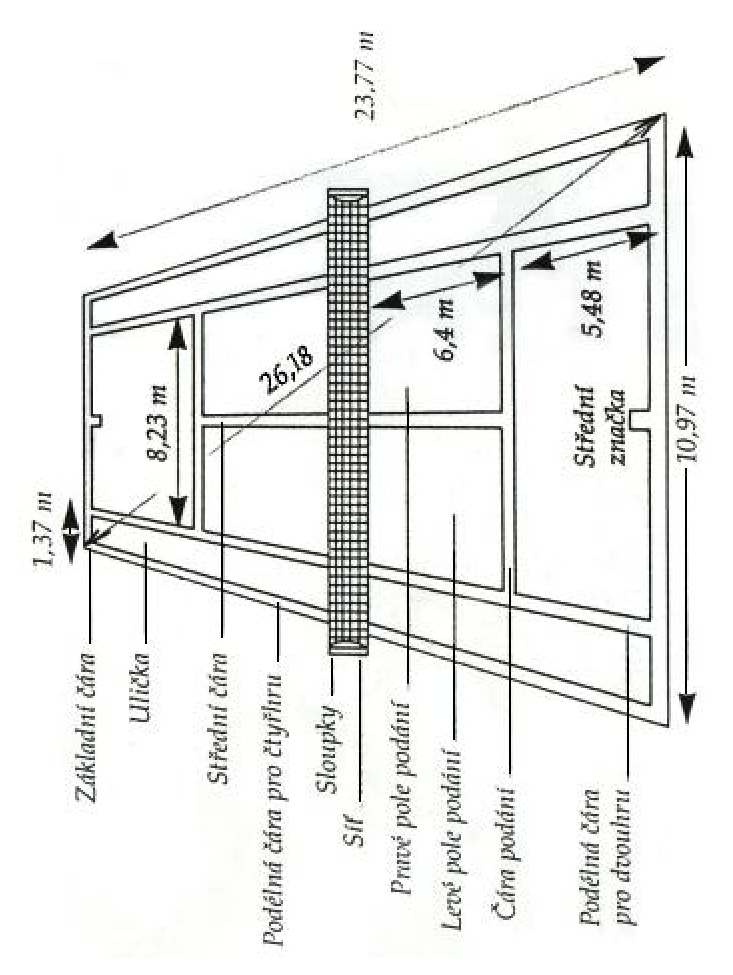
\includegraphics[width=5cm, angle=-90]{hriste.eps}
  \end{center}
  \end{figure}
\end{slide}

\begin{slide}{Použité zdroje:}
  \begin{itemize}
    \item{\url{http://cs.wikipedia.org/wiki/Tenis}}
    \item{\url{http://www.tenis.velesin.cz}}
    \item{\url{http://sokol.bustehrad.sweb.cz/pravidla_tenisu.doc}}
  \end{itemize}
\end{slide}
\end{document}